% ----
% COMP1204 CW1 Report Document
% ----
\documentclass[]{article}

% Reduce the margin size, as they're quite big by default
\usepackage[margin=1in]{geometry}

%Importing fancy package
\usepackage{fancyvrb}
\usepackage[most]{tcolorbox}
\usepackage{xcolor}
\usepackage{graphicx}
\graphicspath{ {./images/} }
\usepackage{blindtext}
\usepackage{soul}
\usepackage[T1]{fontenc}

\title{COMP1204: Data Management \\ Coursework One: Hurricane Monitoring }
% Update these!
\author{Damien Ta \\ 34830294}

% Actually start the report content
\begin{document}

% Add title, author and date info
\maketitle

\section{Introduction}
As data scientists for the National Oceanographic and Atmospheric Administraiton Centre, I was assigned to the tropical cyclone
tracking team. As a data scientist I have been tasked with extracting storm data from the tropical cyclone reports and producing
maps of where the cyclones have taken place.
\clearpage
\section{Create CSV Script}
\subsection{Introduction}
I was tasked with extracting useful data from a set of hurrican reports.
The reports contained lots of information and I coded the \textbf{create\_csv.sh}
script to extract the important information from the reports.
The important information that I extracted included \textbf{Timestamp, Latitude,
Longitude, Minimum Sea Level Pressure and MaxIntensity.}
\subsection{How to run script}
\begin{tcolorbox}[colback=white, colframe=black, boxrule=1pt, arc=2mm, 
    title=Script to run create\_csv.sh, width=6.7in, fonttitle=\bfseries, listing only, listing options={language=sh, basicstyle=\ttfamily}]
\hl{./create\_csv.sh <input\_kml\_file> <output\_csv\_file>}
\begin{verbatim}
This command runs the create_csv.sh file which takes in a kml file and extracts specific
header tag data. The command takes extracted data and saves it to a CSV file.
\end{verbatim}
\end{tcolorbox}
\subsection{Full Script}
\begin{tcolorbox}[colback=white, colframe=black, boxrule=1pt, arc=2mm, 
    title=create\_csv.sh, width=6.7in, fonttitle=\bfseries, listing only, listing options={language=sh, basicstyle=\ttfamily}]
    \begin{verbatim}
1  #!/bin/bash
2  csv_input_path=$1
3  tmp_csv_output=$2
4
5  echo "Timestamp,Latitude,Longitude,MinSeaLevelPressure,MaxIntensity" > $tmp_csv_output
6  dtg="$(grep -R "<dtg>" $csv_input_path | sed 's/.*<dtg>//g' | sed 's/[</dtg>]//g')"
7  grep -R "<lat>" $csv_input_path| sed 's/.*<lat>//g' | sed 's/[</lat>]//g' > lat.csv
8  grep -R "<lon>" $csv_input_path | sed 's/.*<lon>//g' | sed 's/[</lon>]//g' > lon.csv
9  grep -R "<minSeaLevelPres>" $csv_input_path | sed 's/.*<minSeaLevelPres>//g' | /
10 sed 's/[</minSeaLevelPres>]//g' > minSeaLevelPres.csv
11 grep -R "<intensity>" $csv_input_path | sed 's/.*<intensity>//g' | / 
12 sed 's/[</intensity>]//g' > intensity.csv
13 
14 lat="$(sed "s/$/ N/" lat.csv)"
15 lon="$(sed "s/$/ W/" lon.csv)"
16 minSeaLevelPres="$(sed "s/$/ mb/" minSeaLevelPres.csv)"
17 maxIntensity="$(sed "s/$/ knots/" intensity.csv)"
18
19 paste -d',' <(echo "$dtg") <(echo "$lat") <(echo "$lon") <(echo "$minSeaLevelPres") \
20 <(echo "$maxIntensity") >> $tmp_csv_output
21
22 rm lat.csv
23 rm lon.csv
24 rm minSeaLevelPres.csv
25 rm intensity.csv
26 #I used / to continue command on next line
    \end{verbatim}
\end{tcolorbox}
\begin{center}
    Figure 1: create\_csv.sh
\end{center}
\subsection{Script Breakdown}
\subsubsection{Bash Initialization and Passing Arguements into a variable}
\begin{tcolorbox}[colback=white, colframe=black, boxrule=1pt, arc=2mm, 
    title=Bash Initialization and Passing Arguements into a variable, width=6.7in, fonttitle=\bfseries, listing only, listing options={language=sh, basicstyle=\ttfamily}]
    \begin{verbatim}
1 #!/bin/bash
2 csv_input_path=$1
3 tmp_csv_output=$2
    \end{verbatim}
\hl{\#\!/bin/bash}\newline
tells the terminal that when you run the script it should use bash to execute it\newline
\hl{csv\_input\_path=\$1}\newline
\hl{tmp\_csv\_output=\$2}\newline
These two lines of code allow inputs to be enntered into the script
\end{tcolorbox}
\subsubsection{Using grep and sed to filter data of tag headers}
\begin{tcolorbox}[colback=white, colframe=black, boxrule=1pt, arc=2mm, 
    title=Using grep and sed to filter data of tag headers, width=6.7in, fonttitle=\bfseries, listing only, listing options={language=sh, basicstyle=\ttfamily}]
    \begin{verbatim}
5  echo "Timestamp,Latitude,Longitude,MinSeaLevelPressure,MaxIntensity" > $tmp_csv_output
6  dtg="$(grep -R "<dtg>" $csv_input_path | sed 's/.*<dtg>//g' | sed 's/[</dtg>]//g')"
7  grep -R "<lat>" $csv_input_path| sed 's/.*<lat>//g' | sed 's/[</lat>]//g' > lat.csv
8  grep -R "<lon>" $csv_input_path | sed 's/.*<lon>//g' | sed 's/[</lon>]//g' > lon.csv
9  grep -R "<minSeaLevelPres>" $csv_input_path | sed 's/.*<minSeaLevelPres>//g' | \
10 sed 's/[</minSeaLevelPres>]//g' > minSeaLevelPres.csv
11 grep -R "<intensity>" $csv_input_path | sed 's/.*<intensity>//g' | \ 
12 sed 's/[</intensity>]//g' > intensity.csv
    \end{verbatim}
\hl{echo "Timestamp,Latitude,Longitude,MinSeaLevelPressure,MaxIntensity" > \$tmp\_csv\_output}\newline
This command prints the tag headers\newline
\hl{dtg="\$(grep -R "<dtg>" \$csv\_input\_path | sed 's/.*<dtg>//g' | sed 's/[</dtg>]//g')"}\newline
The code creates variable dtg, we grep the kml file inputted at \$1 and search recursively for\newline
keyword <dtg>. The sed 's/.*<dtg>//g' command would replace any character and its occurences \newline
with an empty space including anything before the pattern.\newline
the sed 's/[</dtg>]//g' command would replace any characters between the [], so < / d t g >\newline
to an empty character and the g stands for global.\newline
\hl{grep -R "<lat>" \$csv\_input\_path | sed 's/.*<lat>//g' | sed 's/[</lat>]//g' > lat.csv}\newline
grep recursively keyword <lat> from the kml file inputted\newline
The sed 's/.*<dtg>//g' command would replace any character and its occurences \newline
with an empty space including anything before the pattern.\newline
The sed 's/[</lat>]//g' command would replace any characters between the [ ], so < / l a t >\newline
The outcome is then appended to a file called lat.csv for later use. This same code is then run\newline
on the rest of the tag headers Longitude, MinSeaLevelPressure and MaxIntensity.\newline
\end{tcolorbox}
\subsubsection{Adding units to the end of certain tag headers}
\begin{tcolorbox}[colback=white, colframe=black, boxrule=1pt, arc=2mm, 
    title=Adding units to the end of certain tag headers, width=6.7in, fonttitle=\bfseries, listing only, listing options={language=sh, basicstyle=\ttfamily}]
    \begin{verbatim}
14 lat="$(sed "s/$/ N/" lat.csv)"
15 lon="$(sed "s/$/ W/" lon.csv)"
16 minSeaLevelPres="$(sed "s/$/ mb/" minSeaLevelPres.csv)"
17 maxIntensity="$(sed "s/$/ knots/" intensity.csv)"
    \end{verbatim}
    \hl{lat="\$(sed "s/\$/ N/" lat.csv)"}\newline
    New variable lat is created which uses sed and adds on each line (\$) " N" from file lat.csv\newline
    This is then run on each line of code for longitude, minSeaLevelPres and maxIntensity for their\newline
    respective unit of measure.\newline
\end{tcolorbox}
\subsubsection{Outputting results to file}
\begin{tcolorbox}[colback=white, colframe=black, boxrule=1pt, arc=2mm, 
    title=Outputting results to file, width=6.7in, fonttitle=\bfseries, listing only, listing options={language=sh, basicstyle=\ttfamily}]
    \begin{verbatim}
19 paste -d',' <(echo "$dtg") <(echo "$lat") <(echo "$lon") <(echo "$minSeaLevelPres") /
20 <(echo "$maxIntensity") >> $tmp_csv_output
    \end{verbatim}
\hl{paste -d',' <(echo "\$dtg") <(echo "\$lat") <(echo "\$lon") <(echo "\$minSeaLevelPres") /}\newline
\hl{<(echo "\$maxIntensity") > > \$tmp\_csv\_output}\newline
This code concatenates the variables we created earlier into the file at \$2.\newline
-d',' would add delimiter , after each of the inputs. The < allows you to use an output\newline
of a command as if it were a file.
\end{tcolorbox}
\subsubsection{Removing temporary files from directory}
\begin{tcolorbox}[colback=white, colframe=black, boxrule=1pt, arc=2mm, 
    title=Removing temporary files from directory, width=6.7in, fonttitle=\bfseries, listing only, listing options={language=sh, basicstyle=\ttfamily}]
    \begin{verbatim}
22 rm lat.csv
23 rm lon.csv
24 rm minSeaLevelPres.csv
25 rm intensity.csv
    \end{verbatim}
\hl{rm lat.csv}\newline
rm would remove the file from the current directory. It does this for all temporary files created.
\end{tcolorbox}
\clearpage



\section{Storm Plots}
\subsection{Storm Plot 1}
\begin{figure}[htbp]
    \centering
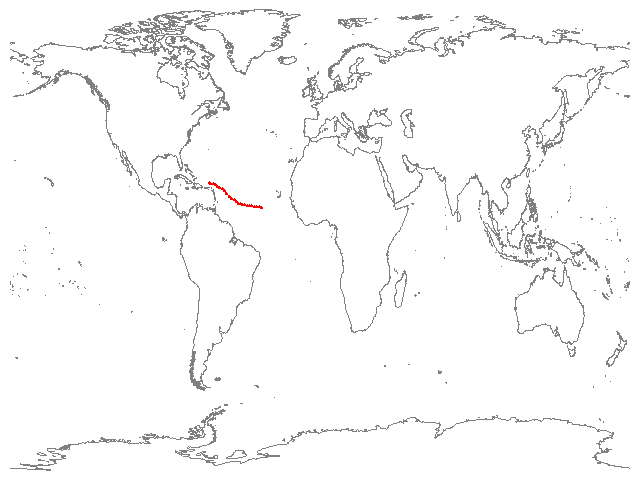
\includegraphics{al112020.png}
\caption{al112020.kml}
\label{fig:al112020}
\end{figure}

\clearpage
\subsection{Storm Plot 2}

\begin{figure}[htbp]
    \centering
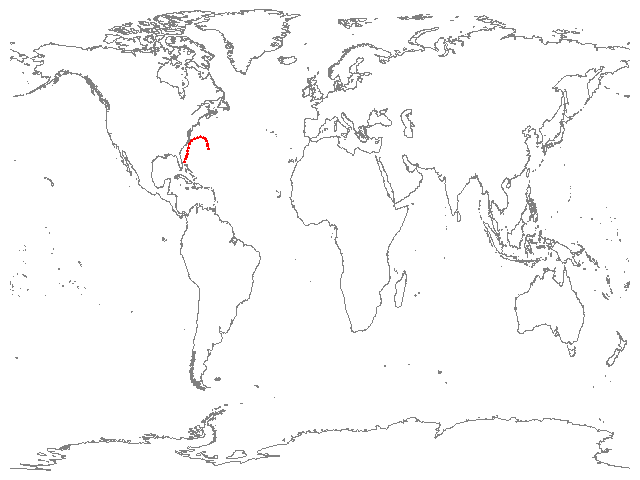
\includegraphics{al012020.png}
\caption{al012020.kml}
\label{fig:al012020}
\end{figure}

\clearpage
\subsection{Storm Plot 3}

\begin{figure}[htbp]
    \centering
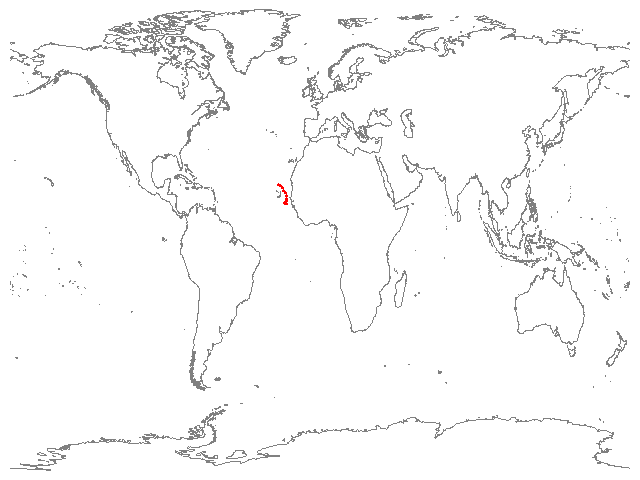
\includegraphics{al102020.png}
\caption{al102020.kml}
\label{fig:al102020}
\end{figure}
\clearpage



\section{Git Usage}
\subsection{Introduction}
I was required to resolve a git conflict that was caused by running the command below. When attempting to merge both branches,
a conflict was created due to the \textbf{python-plot-script.py} file being in two different branches.
\subsection{How to run the conflict script}
The command below ran the script and created a new branch called python-addon and added a file called python-plot-script.py.
\begin{tcolorbox}[colback=white, colframe=black, boxrule=1pt, arc=2mm, 
    fonttitle=\bfseries, listing only, listing options={language=sh, basicstyle=\ttfamily}]
\begin{verbatim}
./conflict-script.sh
\end{verbatim}
\end{tcolorbox}
\subsection{Breakdown of how to fix the conflict}
\subsubsection{Check currrent branch}
First thing I did, was check to see if I was on correct branch and to see if conflict script actually ran
I saw that \textbf{python-addon} was one of the branches meaning the conflict script ran.
\begin{tcolorbox}[colback=white, colframe=black, boxrule=1pt, arc=2mm, 
    fonttitle=\bfseries, listing only, listing options={language=sh, basicstyle=\ttfamily}]
\begin{verbatim}
git branch
\end{verbatim}
\end{tcolorbox}
\subsubsection{Merge the python-addon branch to main branch}
As the conflict script has already run, we were tasked with merging the \textbf{python-addon} branch to the main
branch. We did this using the command below. However, when we attempted to merge the two branches a conflict occured.
\begin{tcolorbox}[colback=white, colframe=black, boxrule=1pt, arc=2mm, 
    fonttitle=\bfseries, listing only, listing options={language=sh, basicstyle=\ttfamily}]
\begin{verbatim}
git merge python-addon
\end{verbatim}
\end{tcolorbox}
\subsubsection{Resolving the conflict}
I opened the \textbf{python-plot-script.py} in my text editor of choice (VSCode) then resolved the conflict by compiling different
parts of each scripts into one script. One of the errors was that we forgot to import math in one of the pieces of code
which I edited. Another error was that in the function \textbf{plot\_all\_csv\_pressure()} one of the scripts had misspelt for and
wrote it as fr. I picked the correct function and moved on. Lastly, the last error I changed was that one of the scripts
was missing a whole function called \textbf{plot\_all\_csv\_intensity()} which I added to the combined script.
\subsubsection{Adding resolved file}
After resolving the conflict, I used the command below to add a change in the working directory to the staging area.
\begin{tcolorbox}[colback=white, colframe=black, boxrule=1pt, arc=2mm, 
    fonttitle=\bfseries, listing only, listing options={language=sh, basicstyle=\ttfamily}]
\begin{verbatim}
git add python-plot-script.py
\end{verbatim}
\clearpage
\end{tcolorbox}
\subsubsection{Commititting the changes}
Committing the changes would save the changes to the local repository. I committed this with an appopriate message about how the
branches have been merged.
\begin{tcolorbox}[colback=white, colframe=black, boxrule=1pt, arc=2mm, 
    fonttitle=\bfseries, listing only, listing options={language=sh, basicstyle=\ttfamily}]
\begin{verbatim}
git commit -am "Merge branch 'python-addon'"
\end{verbatim}
\end{tcolorbox}
\subsubsection{Pushing Changes to Remote Repository}
I uploaded my local repository content to the remote repository 
\begin{tcolorbox}[colback=white, colframe=black, boxrule=1pt, arc=2mm, 
    fonttitle=\bfseries, listing only, listing options={language=sh, basicstyle=\ttfamily}]
\begin{verbatim}
git push origin main
\end{verbatim}
\end{tcolorbox}
\subsection{Final Merged Script}
\begin{tcolorbox}[colback=white, colframe=black, boxrule=1pt, arc=2mm, 
    title=python-plot-script.py, fonttitle=\bfseries, listing only, listing options={language=sh, basicstyle=\ttfamily}]
\begin{verbatim}
1  import pandas as pd
2  import matplotlib.pyplot as plt
3  import os
4  import glob
5  import math
6  user_key = 1773
7   
8  def plot_all_csv_pressure():
9      path = os.getcwd()
10     csv_files = glob.glob(os.path.join(path, '*.csv'))
11        
12     for f in csv_files:
13         storm = pd.read_csv(f)
14         storm['Pressure'].plot()
15         plt.show()
16    
17 def plot_all_csv_intensity():
18     path = os.getcwd()
19     csv_files = glob.glob(os.path.join(path, '*.csv'))
20        
21     for f in csv_files:
22         storm = pd.read_csv(f)
23         storm['Intensity'].plot()
24         plt.show()
\end{verbatim}
\end{tcolorbox}
\begin{center}
    Figure 2: python-plot-script.py
\end{center}

\end{document}
